\subsection{デジタル入力\ruby{装置}{そう|ち}を使ってみよう}
デジタル入力装置をHSPで使ってみましょう。GPIO24にボタン(\#103)をつけてください。HSPスクリプトエディタで\textasciitilde /05/digin.hspを開いて実行してみましょう。\\
\begin{figure}[H]
  \begin{minipage}[t]{0.3\columnwidth}
    \centering
 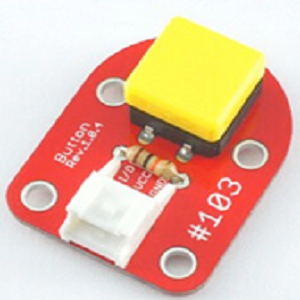
\includegraphics[width=\linewidth]{images/chap05/text05-img028.png}
    \caption{ボタン}
  \end{minipage}
  %\hspace{0.01\columnwidth} % ここで隙間作成
  \begin{minipage}[t]{0.5\columnwidth}
    \centering
    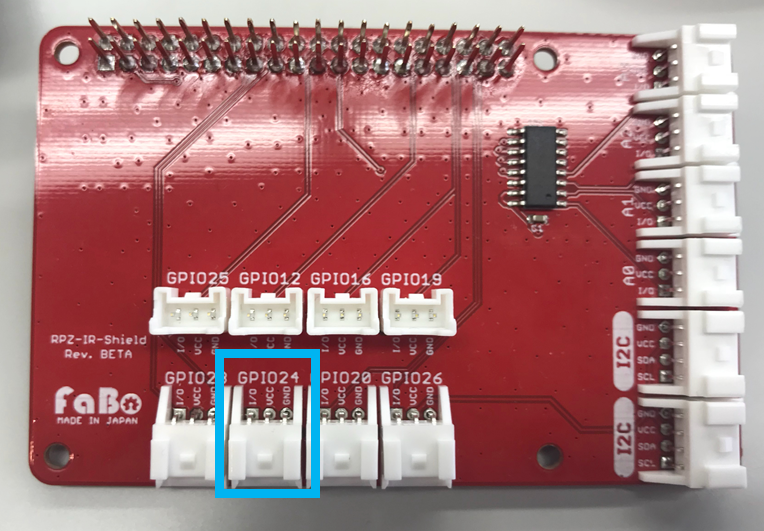
\includegraphics[width=\linewidth]{images/chap05/text05-img029.png}
    \caption{GPIO24}
  \end{minipage}
\end{figure}

\begin{lstlisting}[caption=digout.hsp,label=digout.hsp]
#include "hsp3dish.as"
#include "rpz-gpio.as"

*main
	redraw 0
	pos 30,30
	mes "デジタル入力そうちでLEDを光らせよう"
	redraw 1
	if gpioin(24)=1 : goto *digital_on	<#blue#;GPIO24の値が1のとき*digital_onを実行する#>
	goto *digital_off
        
*digital_on
	gpio 17, 1
	wait 10
	goto *main

*digital_off
	gpio 17, 0
	wait 10
	goto *main
\end{lstlisting}

digin.hspはデジタル入力用のプログラムです。ボタン、スイッチ、リミットスイッチ、\ruby{傾斜}{けい|しゃ}センサーに使うことができます。\\

\code{gpioin(GPIOピン番号)}でデジタル入力を受け取ることができます。\\

\code{if gpioin(24)=1 : goto *digital\_on}でデジタル入力があったとき\code{*digital\_on}に\ruby{移動}{い|どう}します。\code{*digital\_on}では \code{gpio 17, 1}でLEDを光らせています。デジタル入力がないときは \code{goto *digital\_off}で\code{*digital\_off}に移動します。\code{*digital\_off}では \code{gpio 17, 0}でLEDを消しています。

\begin{tcolorbox}[title=\useOmetoi]
\begin{enumerate}
\item ボタン(\#103)をGPIO24につなげて上記のプログラムdigin.hspを実行してみましょう。
\end{enumerate}
\end{tcolorbox}
\begin{tcolorbox}[title=\useOmetoi]
\begin{enumerate}
\addex{スイッチ(\#117)をGPIO24につなげてdigin.hspを実行してみましょう。}
\end{enumerate}
\end{tcolorbox}
\begin{tcolorbox}[title=\useOmetoi]
\begin{enumerate}
\addex{リミットスイッチ(\#107)をGPIO24につなげてdigin.hspを実行してみましょう。}
\end{enumerate}
\end{tcolorbox}
\begin{tcolorbox}[title=\useOmetoi]
\begin{enumerate}
\addex{傾斜センサー(\#110)をGPIO24につなげてdigin.hspを実行してみましょう。}
\end{enumerate}
\end{tcolorbox}
\begin{tcolorbox}[title=\useOmetoi]
\begin{enumerate}
\addex{ボタンをつなげるピンを変えてみましょう。GPIO20にボタン(\#103)をつけましょう。gpioin(24)をgpioin(20)に変えましょう。digin.hspを実行してみましょう。}
\end{enumerate}
\end{tcolorbox}

\begin{tcolorbox}[title=\useOmetoiAlpha]
\begin{enumerate}
\addex{時間があまったら\ruby{挑戦}{ちょう|せん}してみましょう。\\ボタン(\#103)をGPIO26、LED(\#101)をGPIO20につなげます。ボタンを\ruby{押}{お}している間LEDが光るようにdigin.hspを書きかえましょう。}
\end{enumerate}
\end{tcolorbox}
\begin{tcolorbox}[title=\useOmetoiAlpha]
\begin{enumerate}
\addex{時間があまったら挑戦してみましょう。\\ボタンを押して、LEDのONとOFFが切りかわるように、digin.hspを書きかえましょう。}
\end{enumerate}
\end{tcolorbox}
